\section{Replikation bzw. Hedging von Derivaten im CRR-Modell}

Betrachten wir ein Derivat $C$ mit Auszahlung $h(S_1, S_2, \dots, S_N)$ zum Zeitpunkt $N$, d.h. $C = h(S_1, S_2, \dots, S_N)$ mit $h$ messbar.

Gesucht ist nun eine replizierende Strategie $\folge{\xi_n}{n \in \N}$ und eine Anfangskapital $w$, d.h.
\begin{itemize}[label = --, nolistsep, topsep=-\parskip]
	\item $\folge{\xi_n}{n \in \N}$ soll vorhersehbar sein mit diskontiertem Werteprozess $\schlange{\Pi}_n = w + (\xi \bullet \schlange{S})_n$ und 
	\item die Replikationsbedingung soll gelten
	\begin{equation*}
	C = h(S_1, \dots, S_N) = \Pi_N  \qquad \text{fast sicher} \tag{Rep} \label{eq: 2_2_rep}
	\end{equation*}
\end{itemize} 

\begin{*definition}
	\begin{itemize}[nolistsep, topsep=-\parskip]
		\item Ein Derviat $C$ heißt \begriff{erreichbar}, wenn eine Replikationsstrategie existiert.
		\item Ein Finanzmarktmodell heißt \begriff{vollständig}, wenn jedes Derivat erreichbar ist.
	\end{itemize}
\end{*definition}

\begin{satz} %2.3
	\label{satz: 2.2.3}
	Sei $C = h(S_1, \dots, S_N)$ ein Derivat im CRR-Modell. Dann ist $C$ erreichbar, d.h. es existieren $w \in \R$ und $\folge{\xi_n}{n \in \N}$ mit \eqref{eq: 2_2_rep}. Es gilt:
	\begin{itemize}
		\item Es existieren messbare Funktionen $\abb{f_n}{\Rn}{\R}$ für $n =1, \dots, N$, sodass
		\begin{equation*}
			\Pi_n = f_n(S_1, \dots, S_n)
		\end{equation*}
		und die Werte entlang der Pfade des Binomialbaums sind rekursiv bestimmt:
		\begin{align*}
				f_N(S_1, \dots, S_N) &= h(S_1, \dots, S_N) = C \\
				f_n(S_1, \dots, S_n) &= \frac{1}{1+r} \brackets{\frac{r-a}{b-r} f_{n+1}^b + \frac{b-r}{b-a} f_{n+1}^a} \tag{Rek} \label{eq: 2_2_rek}
			\intertext{wobei}
				f_{n+1}^b &= f_{n+1}(S_1, \dots, S_n, S_n (1+b)) \\
				f_{n+1}^a &= f_{n+1}(S_1, \dots, S_n, S_n (1+a))  \qquad (n \in [N]_0)
		\end{align*}		
		\item Die replizierende Strategie ist gegeben durch 
		\begin{equation*}
			\xi_n = \frac{f_n^b - f_n^a}{S_{n-1} (b-a)} \tag{$\Delta$-Hedge} \label{eq: 2_2_dhedge}
		\end{equation*}
	\end{itemize}
\end{satz}

\begin{korollar} %2.4
	Das CRR-Modell ist vollständig.
\end{korollar}

\begin{korollar} %2.5
	Ist $C$ ein europäisches Derivat, d.h. $C = h(S_N)$ mit $\abb{h}{\R}{\R}$ messbar, dann gelten folgende Vereinfachungen: Es reicht $\abb{f_n}{\R}{\R}$ zu wählen und es gilt $\Pi_n = f_n(S_n)$ sowie
	\begin{equation*}
		f_{n+1}^b = f_{n+1}(S_n (1+b)) \quad \und \quad f_{n+1}^a = f_{n+1}(S_n(1+a))
	\end{equation*}
\end{korollar}

\begin{*bemerkung}
	\begin{itemize}[leftmargin=*, label=$\bullet$, nolistsep]
		\item Die Rekursion \eqref{eq: 2_2_rek} entspricht einem Rückwärtsdurchlauf des Baumdiagramms.$f_n$ wird als diskontierter, gewichteter Mittelwert von $f_{n+1}^b$ und $f_{n+1}^a$ bestimmt. Die Gewichte sind dabei $q_b = \frac{r-a}{b-a}$ und $q_a = \frac{b-r}{b-a}$. Es gilt $q_a + q_b = 1$.
		\item Die ursprünglichen Übergangswahrscheinlichkeiten $p$ spielen für Bewertung von $C$ keine Rolle. Sie werden durch die \enquote{risikoneutralen} Wahrscheinlichkeiten $q_b$ und $q_a = 1 - q_b$ ersetzt.
		\item Diese Rekursion lässt sich auf dem Computer auch für große Bäume effizient implementieren.
		\item Die Formel \eqref{eq: 2_2_dhedge} für $\xi_n$ wird auch als Delta-Hedge bezeichnet.
		\begin{equation*}
			\xi_n = \frac{\text{Preisänderung Derivat}}{\text{Preisänderung Basisgut}} \quad \dots \enskip \text{Differenzenquotient}
		\end{equation*}
		\item Weitere Interpretation von $\xi_n$:
		\begin{itemize}
			\item $\xi_n > 0$: Preisänderung Derivat hat selbes Vorzeichen wie Preisänderung Basisgut ; keine Leerverkäufe notwendig.
			\item $\xi_n < 0$: Preisänderung Derivat hat entgegengesetztes Vorzeichen wie Preisänderung Basisgut ; Leerverkäufe sind notwendig.
			\item $\xi_n \approx 0$: Preisänderung Derivat kaum von Preisänderung Basisgut abhängig
		\end{itemize}
	\end{itemize}
\end{*bemerkung}

\begin{proof}[\cref{satz: 2.2.3}]
	Mittels Rückwärtsinduktion über $n \in [N]_0$.
	\begin{description}
		\ianfang Für $n = N$ gilt $\Pi_N = C = h(S_1, \dots, S_N)$ nach \eqref{eq: 2_2_rep}, also $\Pi_N = f_N(S_1, \dots, S_N)$ mit $f_N = h$.
		\ischritt Aus \eqref{eq: sf-schlange} folgt
		\begin{equation*}
			\begin{aligned}
				\schlange{\Pi}_{n+1} - \schlange{\Pi}_n &= \xi_{n+1} \brackets{\schlange{S}_{n+1} - \schlange{S}_n} \qquad\qquad | \ * (1+r)^{n+1} \\
				\follows  \quad \Pi_{n+1} - (1+r) \Pi_n &= \xi_{n+1} \brackets{S_{n+1} - (1+r) S_n}
			\end{aligned} \tag{$\star$} \label{eq: 2_2_3_proof_star}
		\end{equation*}
		Nach Induktionsvoraussetzung gilt also
		\begin{equation*}
			\Pi_{n+1} = f_{n+1} (S_1, \dots, S_{n+1}) = f_{n+1} (S_1, \dots, S_n, S_n (1+R_{n+1}))
		\end{equation*}
		Die zwei Fälle $R_{n+1} = b$ und $R_{n+1} = a$ können jeweils mit strikt positiver Wahrscheinlichkeit eintreten.
		\begin{itemize}
			\item Fall 1: $S_{n+1} = S_n (1+b)$ und $\Pi_{n+1} = f_{n+1}(S_1, \dots, S_n, S_n(1+b)) = f_{n+1}^b$. Setzen wir dies in \eqref{eq: 2_2_3_proof_star} ein, so erhalten wir $f_{n+1}^b - (1+r) \Pi_n = \xi_{n+1} S_n (b-r)$. \hfill (I)
			\item Fall 2: $S_{n+1} = S_n (1+a)$ und $\Pi_{n+1} = f_{n+1}(S_1, \dots, S_n, S_n(1+a)) = f_{n+1}^a$. Setzen wir dies wieder in \eqref{eq: 2_2_3_proof_star} ein, so erhalten wir $f_{n+1}^a - (1+r) \Pi_n = \xi_{n+1} S_n (a-r)$. \hfill (II)
		\end{itemize}
	Damit erhalten wir ein lineares Gleichungssystem [I, II] in den Unbekannten $\Pi_n$ und $\xi_n$. 
	$\Pi_n$ und $\xi_n$ sind $\F_n$-messbar, also unabhängig von $R_{n+1}$. Damit müssen (I) und (II) gleichzeitig erfüllt sein: Subtrahieren wir I -- II, so erhalten wird $f_{n+1}^b - f_{n+1}^a = \xi_{n+1} S_n (b-a)$ und somit folgt \eqref{eq: 2_2_dhedge}
	\begin{equation*}
		\follows \xi_{n+1} = \frac{f_{n+1}^b - f_{n+1}^a}{S_n (b-a)}
	\end{equation*}
	Setzen wir dies wieder in I ein, so erhalten wir
	\begin{equation*}
		f_{n+1}^b - (1+r) \Pi_n = \frac{b-r}{b-a} \brackets{f_{n+1}^b - f_{n+1}^a} \follows \Pi_n = \frac{1}{1+r} \brackets{\frac{r-a}{b-a} f_{n+1}^b + \frac{b-r}{b-a} f_{n+1}^a}
	\end{equation*}
	Dies ist die Rekursionsgleichung \eqref{eq: 2_2_rek}.
	\end{description}
\end{proof}

\begin{*bemerkung}
	Das Lineare Gleichungssystem [I, II] können wir schreiben als
	\begin{equation*}
		\begin{pmatrix}
			1+r & b - r \\
			1+r & a - r \\
		\end{pmatrix}
		* 
		\begin{pmatrix}
			\Pi_n \\ \xi_{n+1} S_n
		\end{pmatrix}
		= 
		\begin{pmatrix}
			f_{n+1}^b \\ f_{n+1}^a
		\end{pmatrix}
		\tag{LGS-1} \label{eq: 2_2_lgs-1}
	\end{equation*}
	Wir können auch ein Trinomialmodell (up, down, gleichbleibender Preis) betrachten. Dabei bekommen wir eine zusätzliche Zeile in obiger Matrix, jedoch ist das Gleichungssystem dann überbestimmt und i.A. nicht mehr eindeutig auflösbar.
\end{*bemerkung}

\begin{*beispiel}[Asiatische Call-Option]
	Die Auszahlung ist gegeben durch 
	\begin{equation*}
		(\quer{S}_N - K)_+ 
		\quad \text{mit} \quad 
		\quer{S}_N = \frac{1}{1+N} \sum_{k=0}^{N} S_k .
	\end{equation*}
	Somit handelt es sich um ein pfadabhängiges Derivat, da die Summe von allen $S_k$ abhängt. 
	Wir bewerten dieses Derivat im CRR-Modell mit zwei Perioden ($N=2$) und Parametern $b = 0.3$, $a = -0.3$, $r=0.1$, $S_0 = 100$, $K=100$. 
	Es gilt $C = h(S_1, S_2)$, also
	
	\begin{center}
		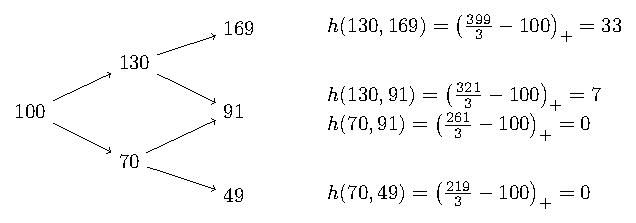
\includegraphics[]{./img/asian-call}
	\end{center}

%	\begin{align*}
%		h(130,169) &= \brackets{\frac{399}{3} - 100}_+ = 33 \\
%		h(130,91)  &= \brackets{\frac{321}{3} - 100}_+ = 7 \\
%		h(70, 91)  &= \brackets{\frac{261}{3} - 100}_+ = 0 \\
%		h(70, 49)  &= \brackets{\frac{219}{3} - 100}_+ = 0 \\
%	\end{align*} 
	
	Außerdem gilt $h = f_2$. Wir berechnen die Übergangswahrscheinlichkeit
	\begin{equation*}
		q = \frac{r-a}{b-a} = \frac{0.4}{0.6} = \frac{2}{3} \follows 1 - q = \frac{1}{3}
	\end{equation*}
	\textbf{Rekursion}
	\begin{align*}
		f_1(130) &= \frac{1}{1+r} \brackets{q * f^b + (1-q) f^a} 
		= \frac{1}{1.1} \brackets{\frac{2}{3} * 33 + \frac{1}{3} * 7} 
		= \frac{1}{1.1} * \frac{73}{3} 
		&&\approx 22.12 \\
		f_1(70) &= \frac{1}{1.1} \brackets{\frac{2}{3} * 0 + \frac{1}{3} * 0} &&= 0 \\
		f_0 &= \frac{1}{1.1} \brackets{\frac{2}{3} * \frac{1}{1.1} * \frac{73}{3} + \frac{1}{3} * 0} = \frac{1}{(1.1)^2} \frac{146}{9} &&\approx 13.41 
	\end{align*}
	\textbf{Strategie}
	\begin{align*}
		\xi_2(130) &= \frac{f_2^b - f_2^a}{S_1 (b-a)} = \frac{33 - 7}{130 * 0.6} = \frac{26}{13*6} &&= \frac{1}{3} \\
		\xi_2(70) &= \frac{0-0}{70 * 0.6} &&= 0 \\
		\xi_1 &= \frac{f_1^b - f_1^a}{S_0 (b-a)} = \frac{\frac{1}{1.1} * \frac{73}{3} - 0}{100 * 0.6} = \frac{73}{2*11*6} = \frac{73}{196} &&\approx 0.37
	\end{align*}
\end{*beispiel}


